\chapter{Technologie}
\label{chap:technologie}

\section{MQTT}

\textit{Die folgende Einführung des MQTT Protokolls wurde aus der dem Ergebnis des BFH Modul BTI7302 (Projekt 2) von Adrian Bärtschi übernommen.}

MQTT (Message Queue Telemetry Transport) ist ein Netzwerkprotokoll, das sich dank einfachem und leichtgewichtigen Design sehr gut für Geräte mit stark eingeschränkten Ressourcen und Netzwerke mit geringer Bandbreite eignet. 
\\
Die erste Version von MQTT wurde 1999 von Dr. Andy Stanford-Clark (IBM) und Arlen Nipper (Arcom) beschrieben und entwickelt. Inzwischen ist MQTT in der Version 3.1.1 verfügbar  \cite{mqttSpez} und wird von OASIS Konsortium (\url{https://www.oasis-open.org}) standardisiert.

Im OSI Modell ist MQTT auf dem Application Layer eingeordnet, basierend auf dem TCP Stack.

\begin{figure}[H]
	\centering
		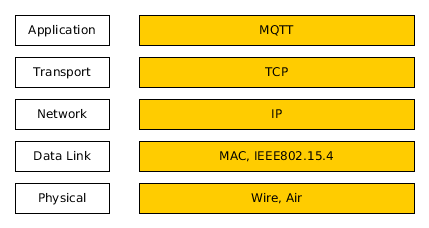
\includegraphics[width=0.6\textwidth]{diag/osi_mqtt.png}
	\caption{\label{fig:mqttosi}MQTT im (vereinfachten) OSI Stack}
\end{figure}

\subsection{Publish/Subscribe}
MQTT funktioniert nach dem Publish/Subscribe Pattern. Im Gegensatz zum klassichen Client/Server Prinzip registrieren sich die Clients (Subscriber) bei einem Broker für bestimmte Bereiche (Topics), zu denen sie Nachrichten erhalten möchten.
\\ \\

\begin{figure}[H]
	\centering
		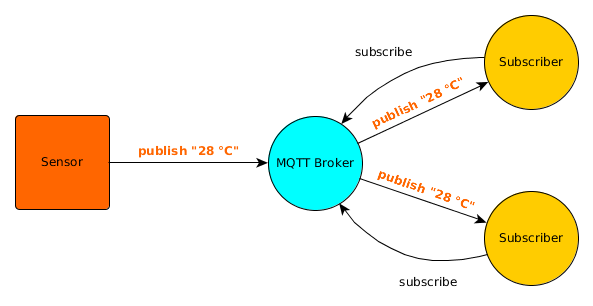
\includegraphics[width=0.8\textwidth]{diag/pub_sub.png}
	\caption{\label{fig:pub_sub}Publish/Subscribe Prinzip}
\end{figure}


\par
Ein Publisher, (z. Bsp. ein Sensor) sendet seine Nachrichten an den Broker. Alle Subscriber, die sich für das entsprechende Topic eingeschrieben haben, erhalten die Nachricht vom Broker. 
\\ \\
Diese Entkopplung der Teilnemhner bringt diverse Vorteile mit sich:

\begin{itemize}
\item Publisher und Subscriber müssen sich gegenseitig nicht kennen
\item Clients können sich beliebig an- und abmelden
\item Beim Ausfall eines Teilnehmers sind die anderen nicht blockiert
\end{itemize}

\subsection{Topics}
Jede Nachricht wird an ein bestimmtes Topic gesendet. Grundsätzlich kann jeder Client zu jedem Topic des Brokers Nachristen veröffentlichen. Die Topics sind hierarchisch aufgebaut, die Ebenen werden durch einen Slash (/) getrennt.\\
Zum Beispiel könnte ein Thermometer seine Temperatur im Topic \texttt{house/livingroom/temperature} veröffentlichen.\\ \\
Um die Nachrichten zu erhalten, muss sich nun ein anderer Client für dieses Topic einschreiben. Dabei können die Wildcards \texttt{+} und \texttt{\#} verwendet werden.\\
Das \texttt{+} Symbol steht für eine Ebene in der Topic Hierarchie.\\
Beispiel: \texttt{house/+/temperature} steht für die Temperaturmeldungen aller Räume des Hauses .

\begin{itemize}
	\item \texttt{house/livingroom/temperature}
    \item \texttt{house/kitchen/temperature}
    \item \texttt{house/bedroom/temperature}
    \item \texttt{...}
\end{itemize}

Mit \texttt{\#} werden alle Topics des Unterbaums abonniert.
Beispiel: Wenn ein Client das Topic \texttt{house/\#} abonniert, erhält dieser alle Meldungen des Hauses.

\begin{itemize}
	\item \texttt{house/bedroom/temperature}
    \item \texttt{house/door/status}
    \item \texttt{...}
\end{itemize}

\subsection{Messages}
Messages in MQTT sind sehr einfach aufgebaut. Eine Message hat folgende Attribute:\\

\begin{table}[h!]
\centering
\begin{tabular}{ |l|l| }
	\hline
	Attribut & Beschreibung \\ 
	\hline
	Payload    	& Beliebige Daten im Binärformat. Maximal 256 MB     \\
	QoS    		& Quality of Service 0, 1 oder 2. Details in Kapitel \ref{qos}    \\ 
	Retained    & Flag, true oder false, Details in Kapitel \ref{retained}     \\ 
	\hline
\end{tabular}
\caption{Aufbau einer MQTT Message}
\end{table}


\subsection{Quality of Service} \label{qos}
MQTT bietet drei verschiedene QoS Einstellungen für das versenden von Nachrichten.
\begin{itemize}
\item 0: Die Nachricht wird einmal versendet, es gibt keine Bestätigung des Empfängers.
\item 1: (Standard) Die Nachricht wird mindestens einmal beim Empfänger ankommen. Es wird so lange versucht zu senden, bis eine Bestätigung erhalten wurde.
\item 2: Mit ein Handhshake Mechanismus wird sichergestellt, dass die Nachricht genau einmal beim Empfänger angekommen ist.
\end{itemize}

Je höher die QoS Einstellung, desto mehr Resourcen werden beim versenden benötigt und es desto mehr Daten werden über das Netzwerk gesendet.

\subsection{Retaines Messages} \label{retained}
Bei einer MQTT Message kann das Retained Flag gesetzt werden. Damit wird pro Topic die letzte Nachricht auf dem Broker gespeichert. Verbindet sich ein neuer Client und abonniert das Topic, erhält er die retained Message sofort. Dies kann nützlich sien bei Anwendungen mit Topics, die sehr lange Pausen zwischen den Meldungen haben.

\subsection{Last Will}
Jeder Client, der sich zum Broker vebindet, kann eine ''Last Will'' Message angeben. Diese Meldung wird an das gewünschte Topic gesendet, sobald die Verbindung beendet wird.

\pagebreak

\subsection{Implementationen}
Inzwischen sind zahlreiche Implementationen von sowohl MQTT Brokern, als auch Client Libraries verfügbar.

\paragraph{Broker}

\begin{center}
\begin{tabular}{ | m{5em} | m{25em}| m{12em} | }
 \hline
 Name & Beschreibung & URL \\
 \hline
 Mosquitto  & Leichtgewichtiger Open Source Broker geschrieben in C. Zurzeit de-facto standard MQTT Broker. & \url{http://mosquitto.org/}  \\
 \hline
 ActiveMQ Apollo   & OSS Message Broker, untersützt neben MQTT noch andere Protokolle. Konfiguration und Administration über Web GUI. & \url{http://activemq.apache.org/apollo/}  \\
  \hline
 Moquette  & OSS Broker Implementation in Java. Kann auch als Library in eigene Projekte eingebunden werden. & \url{https://github.com/andsel/moquette}  \\
 \hline
  HiveMQ  & Proprietärer MQTT Broker, ausgerichtet für Enterprise Anwendungen.  & \url{http://www.hivemq.com/}  \\
 \hline
  Mosca  & MQTT Broker für die NodeJS Platform. Kann als Standalone oder Embedded Broker verwendet werden.  & \url{http://www.mosca.io/}  \\
\hline

\end{tabular}
\end{center}



\paragraph{Client Libraries}

Das Eclipse Projekt Paho \cite{paho} stellt Client Libraries für C, Java, Android, Python,
 Javascript, C/C++ embedded und .Net / WinRT zur verfügung. Die Java Library sich als stabil und gut dokumentiert erwiesen.

Eine Lister mit weiteren Client Libraries ist im MQTT Wiki \cite{clientLibs} zu finden.



\section{Bestehende Konzepte}
Die verschiedenen Hersteller von MQTT Anwendungen entwickeln jeweils ihre eigenen Ansätze, um die Daten zu strukturieren. 


\subsection{IBM Internet of Things Foundation}

IBM hat unter dem Brand `IBM IoT Foundation' \cite{ibmIotF:home} einen Dienst entwickelt, mit dem vernetzte Geräte verwaltet werden können. Als Kommunikationsprotokoll wird MQTT eingesetzt. Die Plattform verwendet folgende konzeptionelle Ideen:
\begin{itemize}
    \item Organizations: Eindeutige Identifikation der Kunden der Plattform
	\item Devices: Beliebiges vernetztes Gerät. Versendet Events und reagiert auf Commands.
	\item Applications: Anwendung, welche mit den Daten der Devices interagiert.
	\item Events: Daten, welche von den Devices an die Plattform gesendet werden
	\item Commands: Applications können mittels Commands mit den Devices kommunizieren.
\end{itemize}

\textbf{Events} \\
Events müssen an ein definiertes Topic nach folgendem Schema gesendet werden: \\
\code{iot-2/evt/<event\_id>/fmt/<format\_string>}

Beispiel: \code{iot-2/evt/temperature\_outdoor/fmt/json}

Eine Anwendung, welche Events empfangen möchte, muss sich auf ein Topic in der Form \\
\code{iot-2/type/<device\_type>/id/<device\_id>/evt/<event\_id>/fmt/<format\_string>} registrieren.
Die Teile \code{device\_type}, \code{device\_id}, \code{event\_id} und \code{format\_string} des Topics können auch mit dem Wildcard Charakter '\code{+}' ersetzt werden, um jeweils alle Events der Komponenten zu erhalten. 

Beispiel: \code{iot-2/type/temp/id/+/evt/temperature\_outdoor/fmt/+}

\textbf{Commands} \\
Um einen Command zu erzeugen, sendet eine Anwendung eine MQTT Message mit Topic gemäss folgenden Schema:
\code{iot-2/type/<device\_type>/id/<device\_id>/cmd/<command\_id>/fmt/<format\_string>}

Beispiel: \code{iot-2/type/temp/id/sensor1/cmd/setInterval/fmt/json}

Das Device \code{sensor1} würde damit eine Message auf Topic \code{iot-2/cmd/setInterval/fmt/json} erhalten.


\textbf{Payload Format} \\
Grundsätzlich unterstützt IBM IoT Foundation ein beliebiges Payload Format. Es wird jedoch empfohlem, JSON zu verwenden. Um alle Funktionen der Platform nutzen zu können, müssen die JSON Dokumente zusätzlich nach den Vorgaben \cite{ibmIotF:payload} von IBM strukturiert sein.

\begin{listing}[H]
\begin{minted}[frame=single,
               framesep=3mm,
               linenos=false,
               xleftmargin=21pt,
               tabsize=4]{json}
{
  "d": {
    "host": "IBM700-R9E683D",
    "mem": 54.9,
    "network": {
      "up": 1.22,
      "down": 0.55
    },
    "cpu": 1.3,
  }
}
\end{minted}
\caption{JSON Beispiel im IBM IoTF Payload Format}
\end{listing}
\begin{minted}{json}
\end{minted}


\subsection{Tinkerforge MQTT Proxy}

Tinkerforge hat ein modulares System von Sensoren und Aktoren (so gennate Bricklets) entwickelt, die u. A. für Prototyping und in der Ausbildung (auch an der BFH) eingesetzt werden. Um die Mudule zu steuern, wird klassischerweise das bereitstellete SDK in der gewünschten Programmiersprache verwendet. 
Tinkerforge ausserdem eine Anwendung entwickelt und die Bausteine per MQTT ansprechen zu können \cite{tinkerf:mqtt}.

\textbf{Topics} \\
Die Tinkerforge Devices senden ihre Daten an ein MQTT Topic nach Schema \\ \code{tinkerforge/<prefix>/<uid>/<suffix>}.

Ein Temperatur Bricklet mit \acrfull{uid} \code{xf2} würde also den gemessenen Wert an das Topic \\
\code{tinkerforge/bricklet/temperature/xf2/temperature} senden.

Die Bricklets reagieren auf Messages die an ein passendes Topic mit Siffix \code{/set} gesendet werden. Sollen beispielsweise die LEDs des Dualbutton Bricklets mit UID \code{mxg} eingeschaltet werden, muss eine Message an das Topic \code{tinkerforge/bricklet/dual\_button/mxg/led\_state/set} gesendet werden mit folgendem Payload:

\begin{listing}[H]
\begin{minted}[frame=single,
               framesep=3mm,
               linenos=false,
               xleftmargin=21pt,
               tabsize=4]{json}
{
    "led_l": 2,
    "led_r": 2
}
\end{minted}
\caption{JSON Beispiel Tinkerforge Format}
\end{listing}
\begin{minted}{json}
\end{minted}


\textbf{Payload Format} \\
Die Tinkerforge MQTT Komponente verwendet JSON als Datenformat für die Messages. Jede Message, die von einem Bricklet gesendet wird, enthält unter dem Key \code{\_timestamp} den Zeitpunkt der Erzeugung als UNIX Timestamp.

\begin{listing}[H]
\begin{minted}[frame=single,
               framesep=3mm,
               linenos=false,
               xleftmargin=21pt,
               tabsize=4]{json}
{
  "_timestamp": 1440083842.785104,
  "temperature": 2343
}
\end{minted}
\caption{JSON Beispiel Tinkerforge Format}
\end{listing}
\begin{minted}{json}
\end{minted}

Die Beschreibung, unter welchen Topics Daten publiziert werden und wie die Bricklets angesprochen werden können, ist in der Dokumentation von Tinkerforge \cite{tinkerf:mqtt} beschrieben.


\section{Datenbeschreibung}

\subsection{JSON Schema}

\subsection{Protocol Buffer}

\subsection{DFDL}
Aus Proj2 übernehmen

\subsection{Vergleich}



% \section{CoAP?}

% \section{Eclipse Vorto}
% https://www.eclipse.org/vorto/index.html

% \section{OMA LWM2M - Leshan}
% https://eclipse.org/leshan/

\section{Konzept aus der nicht-IoT Welt}
SOAP-WSDL, REST, etc.
HATEOAS
